\hypertarget{mtk__glpk__adapter_8cc}{\section{src/mtk\-\_\-glpk\-\_\-adapter.cc File Reference}
\label{mtk__glpk__adapter_8cc}\index{src/mtk\-\_\-glpk\-\_\-adapter.\-cc@{src/mtk\-\_\-glpk\-\_\-adapter.\-cc}}
}


Adapter class for the G\-L\-P\-K A\-P\-I.  


{\ttfamily \#include $<$cmath$>$}\\*
{\ttfamily \#include $<$cstring$>$}\\*
{\ttfamily \#include $<$iostream$>$}\\*
{\ttfamily \#include $<$iomanip$>$}\\*
{\ttfamily \#include $<$limits$>$}\\*
{\ttfamily \#include \char`\"{}mtk\-\_\-roots.\-h\char`\"{}}\\*
{\ttfamily \#include \char`\"{}mtk\-\_\-blas\-\_\-adapter.\-h\char`\"{}}\\*
{\ttfamily \#include \char`\"{}mtk\-\_\-glpk\-\_\-adapter.\-h\char`\"{}}\\*
Include dependency graph for mtk\-\_\-glpk\-\_\-adapter.\-cc\-:\nopagebreak
\begin{figure}[H]
\begin{center}
\leavevmode
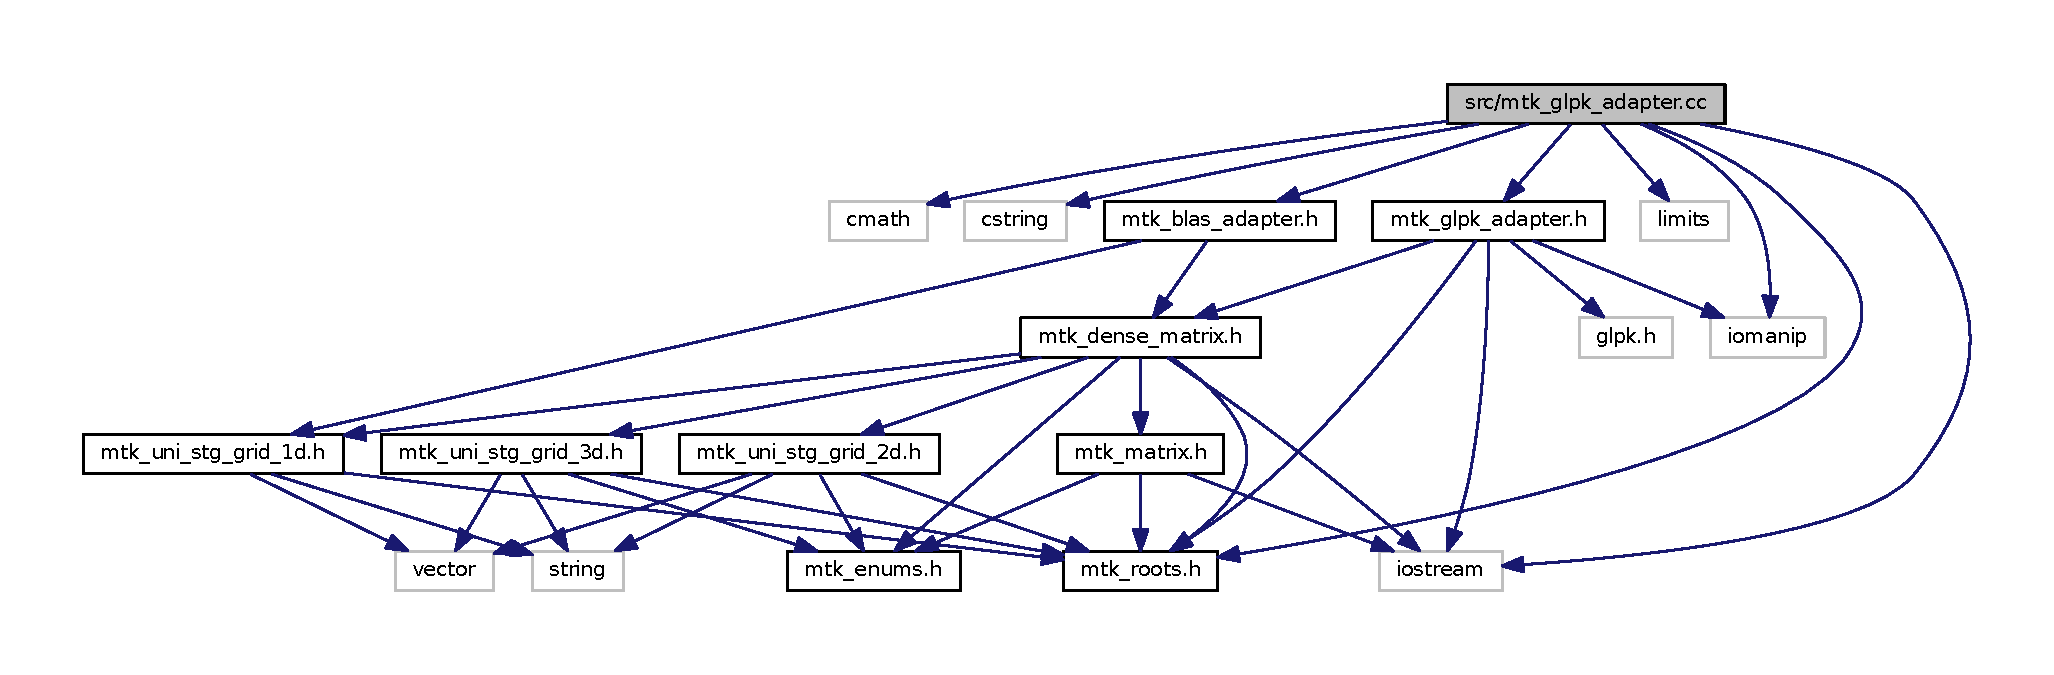
\includegraphics[width=350pt]{mtk__glpk__adapter_8cc__incl}
\end{center}
\end{figure}


\subsection{Detailed Description}
This class contains a collection of static classes, that posses direct access to the underlying structure of the matrices, thus allowing programmers to exploit some of the numerical methods implemented in the G\-L\-P\-K.

The {\bfseries G\-L\-P\-K (G\-N\-U Linear Programming Kit)} package is intended for solving large-\/scale linear programming (L\-P), mixed integer programming (M\-I\-P), and other related problems. It is a set of routines written in A\-N\-S\-I C and organized in the form of a callable library.

\begin{DoxySeeAlso}{See Also}
\href{http://www.gnu.org/software/glpk/}{\tt http\-://www.\-gnu.\-org/software/glpk/}
\end{DoxySeeAlso}
\begin{DoxyAuthor}{Author}
\-: Eduardo J. Sanchez (ejspeiro) -\/ esanchez at mail dot sdsu dot edu 
\end{DoxyAuthor}


Definition in file \hyperlink{mtk__glpk__adapter_8cc_source}{mtk\-\_\-glpk\-\_\-adapter.\-cc}.

